% Options for packages loaded elsewhere
% Options for packages loaded elsewhere
\PassOptionsToPackage{unicode}{hyperref}
\PassOptionsToPackage{hyphens}{url}
\PassOptionsToPackage{dvipsnames,svgnames,x11names}{xcolor}
%
\documentclass[
  default,
]{sn-jnl}


\usepackage{xcolor}
\usepackage{amsmath,amssymb}
\setcounter{secnumdepth}{5}
\usepackage{iftex}
\ifPDFTeX
  \usepackage[T1]{fontenc}
  \usepackage[utf8]{inputenc}
  \usepackage{textcomp} % provide euro and other symbols
\else % if luatex or xetex
  \usepackage{unicode-math} % this also loads fontspec
  \defaultfontfeatures{Scale=MatchLowercase}
  \defaultfontfeatures[\rmfamily]{Ligatures=TeX,Scale=1}
\fi
\usepackage{lmodern}
\ifPDFTeX\else
  % xetex/luatex font selection
\fi
% Use upquote if available, for straight quotes in verbatim environments
\IfFileExists{upquote.sty}{\usepackage{upquote}}{}
\IfFileExists{microtype.sty}{% use microtype if available
  \usepackage[]{microtype}
  \UseMicrotypeSet[protrusion]{basicmath} % disable protrusion for tt fonts
}{}
\makeatletter
\@ifundefined{KOMAClassName}{% if non-KOMA class
  \IfFileExists{parskip.sty}{%
    \usepackage{parskip}
  }{% else
    \setlength{\parindent}{0pt}
    \setlength{\parskip}{6pt plus 2pt minus 1pt}}
}{% if KOMA class
  \KOMAoptions{parskip=half}}
\makeatother
% Make \paragraph and \subparagraph free-standing
\makeatletter
\ifx\paragraph\undefined\else
  \let\oldparagraph\paragraph
  \renewcommand{\paragraph}{
    \@ifstar
      \xxxParagraphStar
      \xxxParagraphNoStar
  }
  \newcommand{\xxxParagraphStar}[1]{\oldparagraph*{#1}\mbox{}}
  \newcommand{\xxxParagraphNoStar}[1]{\oldparagraph{#1}\mbox{}}
\fi
\ifx\subparagraph\undefined\else
  \let\oldsubparagraph\subparagraph
  \renewcommand{\subparagraph}{
    \@ifstar
      \xxxSubParagraphStar
      \xxxSubParagraphNoStar
  }
  \newcommand{\xxxSubParagraphStar}[1]{\oldsubparagraph*{#1}\mbox{}}
  \newcommand{\xxxSubParagraphNoStar}[1]{\oldsubparagraph{#1}\mbox{}}
\fi
\makeatother


\usepackage{longtable,booktabs,array}
\usepackage{calc} % for calculating minipage widths
% Correct order of tables after \paragraph or \subparagraph
\usepackage{etoolbox}
\makeatletter
\patchcmd\longtable{\par}{\if@noskipsec\mbox{}\fi\par}{}{}
\makeatother
% Allow footnotes in longtable head/foot
\IfFileExists{footnotehyper.sty}{\usepackage{footnotehyper}}{\usepackage{footnote}}
\makesavenoteenv{longtable}
\usepackage{graphicx}
\makeatletter
\newsavebox\pandoc@box
\newcommand*\pandocbounded[1]{% scales image to fit in text height/width
  \sbox\pandoc@box{#1}%
  \Gscale@div\@tempa{\textheight}{\dimexpr\ht\pandoc@box+\dp\pandoc@box\relax}%
  \Gscale@div\@tempb{\linewidth}{\wd\pandoc@box}%
  \ifdim\@tempb\p@<\@tempa\p@\let\@tempa\@tempb\fi% select the smaller of both
  \ifdim\@tempa\p@<\p@\scalebox{\@tempa}{\usebox\pandoc@box}%
  \else\usebox{\pandoc@box}%
  \fi%
}
% Set default figure placement to htbp
\def\fps@figure{htbp}
\makeatother


% definitions for citeproc citations
\NewDocumentCommand\citeproctext{}{}
\NewDocumentCommand\citeproc{mm}{%
  \begingroup\def\citeproctext{#2}\cite{#1}\endgroup}
\makeatletter
 % allow citations to break across lines
 \let\@cite@ofmt\@firstofone
 % avoid brackets around text for \cite:
 \def\@biblabel#1{}
 \def\@cite#1#2{{#1\if@tempswa , #2\fi}}
\makeatother
\newlength{\cslhangindent}
\setlength{\cslhangindent}{1.5em}
\newlength{\csllabelwidth}
\setlength{\csllabelwidth}{3em}
\newenvironment{CSLReferences}[2] % #1 hanging-indent, #2 entry-spacing
 {\begin{list}{}{%
  \setlength{\itemindent}{0pt}
  \setlength{\leftmargin}{0pt}
  \setlength{\parsep}{0pt}
  % turn on hanging indent if param 1 is 1
  \ifodd #1
   \setlength{\leftmargin}{\cslhangindent}
   \setlength{\itemindent}{-1\cslhangindent}
  \fi
  % set entry spacing
  \setlength{\itemsep}{#2\baselineskip}}}
 {\end{list}}
\usepackage{calc}
\newcommand{\CSLBlock}[1]{\hfill\break\parbox[t]{\linewidth}{\strut\ignorespaces#1\strut}}
\newcommand{\CSLLeftMargin}[1]{\parbox[t]{\csllabelwidth}{\strut#1\strut}}
\newcommand{\CSLRightInline}[1]{\parbox[t]{\linewidth - \csllabelwidth}{\strut#1\strut}}
\newcommand{\CSLIndent}[1]{\hspace{\cslhangindent}#1}



\setlength{\emergencystretch}{3em} % prevent overfull lines

\providecommand{\tightlist}{%
  \setlength{\itemsep}{0pt}\setlength{\parskip}{0pt}}





%%%% Standard Packages

\usepackage{graphicx}%
\usepackage{multirow}%
\usepackage{amsmath,amssymb,amsfonts}%
\usepackage{amsthm}%
\usepackage{mathrsfs}%
\usepackage[title]{appendix}%
\usepackage{xcolor}%
\usepackage{textcomp}%
\usepackage{manyfoot}%
\usepackage{booktabs}%
\usepackage{algorithm}%
\usepackage{algorithmicx}%
\usepackage{algpseudocode}%
\usepackage{listings}%

%%%%

\raggedbottom
\makeatletter
\@ifpackageloaded{caption}{}{\usepackage{caption}}
\AtBeginDocument{%
\ifdefined\contentsname
  \renewcommand*\contentsname{Table of contents}
\else
  \newcommand\contentsname{Table of contents}
\fi
\ifdefined\listfigurename
  \renewcommand*\listfigurename{List of Figures}
\else
  \newcommand\listfigurename{List of Figures}
\fi
\ifdefined\listtablename
  \renewcommand*\listtablename{List of Tables}
\else
  \newcommand\listtablename{List of Tables}
\fi
\ifdefined\figurename
  \renewcommand*\figurename{Figure}
\else
  \newcommand\figurename{Figure}
\fi
\ifdefined\tablename
  \renewcommand*\tablename{Table}
\else
  \newcommand\tablename{Table}
\fi
}
\@ifpackageloaded{float}{}{\usepackage{float}}
\floatstyle{ruled}
\@ifundefined{c@chapter}{\newfloat{codelisting}{h}{lop}}{\newfloat{codelisting}{h}{lop}[chapter]}
\floatname{codelisting}{Listing}
\newcommand*\listoflistings{\listof{codelisting}{List of Listings}}
\makeatother
\makeatletter
\makeatother
\makeatletter
\@ifpackageloaded{caption}{}{\usepackage{caption}}
\@ifpackageloaded{subcaption}{}{\usepackage{subcaption}}
\makeatother
\makeatletter
\@ifpackageloaded{sidenotes}{}{\usepackage{sidenotes}}
\@ifpackageloaded{marginnote}{}{\usepackage{marginnote}}
\makeatother
\usepackage{bookmark}
\IfFileExists{xurl.sty}{\usepackage{xurl}}{} % add URL line breaks if available
\urlstyle{same}
\hypersetup{
  pdftitle={Chapter 4 - Procedure for testing and adjusting translations of the Soundscape (quasi-)Circumplex Model},
  pdfauthor={Andrew Mitchell; Francesco Aletta},
  colorlinks=true,
  linkcolor={blue},
  filecolor={Maroon},
  citecolor={Blue},
  urlcolor={Blue},
  pdfcreator={LaTeX via pandoc}}


\title[Chapter 4 - Procedure for testing and adjusting translations of
the Soundscape (quasi-)Circumplex Model]{Chapter 4 - Procedure for
testing and adjusting translations of the Soundscape (quasi-)Circumplex
Model}

% author setup
\author*[1]{\fnm{Andrew} \sur{Mitchell}}\email{andrew.mitchell.18@ucl.ac.uk}\author[1]{\fnm{Francesco} \sur{Aletta}}\email{f.aletta@ucl.ac.uk}
% affil setup
\affil[1]{\orgdiv{Institute for Environmental Design and
Engineering}, \orgname{University College
London}, \orgaddress{\street{Central House, 14 Upper Woburn
Place}, \city{London}, \postcode{WC1H 0NN}}}

% abstract 

\abstract{This chapter outlines a systematic procedure for evaluating
and normalising the structure of translated versions of the Soundscape
Circumplex Model (SCM) questionnaire. A four-step approach is proposed
to assess the quasi-circumplex structure of translated instruments,
identify deviations from the original model, and implement corrective
measures to enhance structural fidelity. The results are presented with
a three-tier confidence level system (Low, Medium, High) to indicate the
reliability of the circumplex structure in the translated versions. To
enable normalisation across different translations of the circumplex
attributes, ``adjusted angles'' are derived, which are a measure
proposed to correct the SCM structure (i.e., the pleasant-eventful
coordinate space proposed in the ISO 12913 series) of a given language.

Results reveal that most languages successfully maintain the
quasi-circumplex structure of the original soundscape model, ensuring
robust cross-cultural validity.

\ldots{}}

% keywords

\begin{document}
\maketitle


\section{Introduction}\label{introduction}

In the following chapters, case studies of individual languages are
presented, demonstrating an array of approaches to evaluating the
validity of proposed translations. This diversity of translation and
evaluation methodologies allows for a nuanced understanding of the
particular challenges inherent to each language and translation attempt.
However, to ensure consistency and comparability across all nineteen
languages, it was necessary to develop a standardised quantitative
procedure which can evaluate all languages on the same basis and
consider the compiled dataset as a whole.

This chapter therefore presents a systematic procedure for evaluating
and adjusting the quasi-circumplex structure of translated versions of
the Soundscape Circumplex Model (SCM) questionnaire. The procedure
consists of four key steps: (1) testing for the presence of a
quasi-circumplex structure in the translated instrument, (2) assessing
the fit of the circumplex model to the data, (3) identifying deviations
from the original model, and (4) implementing corrective measures to
enhance structural fidelity and normalisation across translations.

We begin with a brief overview of the circumplex model and its relevance
to psychometrics, followed by a detailed description of the proposed
procedure. The chapter concludes with a discussion on the assessed
validity of each translation and the implications of the findings for
cross-cultural research in soundscape studies.

\section{Defining the circumplex
model}\label{defining-the-circumplex-model}

The concept of the psychometric circumplex model, first introduced by
Guttman (1954), revolves around the idea of a circular relationship
among variables. This circular relationship can be seen by identifying
certain correlation patterns within the correlation matrix among
variables, when appropriately ordered (Browne 1992). In the case of the
circular structure, the strength of the correlation coefficients in the
matrix decreases as you move away from the diagonal, and then increases
again as you move towards the opposite diagonal. This pattern of
correlations can be seen in Table~\ref{tbl-circumplex}.

\begin{longtable}[]{@{}
  >{\raggedright\arraybackslash}p{(\linewidth - 16\tabcolsep) * \real{0.0714}}
  >{\raggedright\arraybackslash}p{(\linewidth - 16\tabcolsep) * \real{0.1122}}
  >{\raggedright\arraybackslash}p{(\linewidth - 16\tabcolsep) * \real{0.1122}}
  >{\raggedright\arraybackslash}p{(\linewidth - 16\tabcolsep) * \real{0.1122}}
  >{\raggedright\arraybackslash}p{(\linewidth - 16\tabcolsep) * \real{0.1122}}
  >{\raggedright\arraybackslash}p{(\linewidth - 16\tabcolsep) * \real{0.1122}}
  >{\raggedright\arraybackslash}p{(\linewidth - 16\tabcolsep) * \real{0.1122}}
  >{\raggedright\arraybackslash}p{(\linewidth - 16\tabcolsep) * \real{0.1122}}
  >{\raggedright\arraybackslash}p{(\linewidth - 16\tabcolsep) * \real{0.0714}}@{}}
\caption{Theoretical pattern of the correlation matrix corresponding to
a circular structure. \(\rho_1 > \rho_2 > \rho_3 > \rho_4\) (Gurtman and
Pincus 2000).}\label{tbl-circumplex}\tabularnewline
\toprule\noalign{}
\begin{minipage}[b]{\linewidth}\raggedright
\end{minipage} & \begin{minipage}[b]{\linewidth}\raggedright
V1
\end{minipage} & \begin{minipage}[b]{\linewidth}\raggedright
V2
\end{minipage} & \begin{minipage}[b]{\linewidth}\raggedright
V3
\end{minipage} & \begin{minipage}[b]{\linewidth}\raggedright
V4
\end{minipage} & \begin{minipage}[b]{\linewidth}\raggedright
V5
\end{minipage} & \begin{minipage}[b]{\linewidth}\raggedright
V6
\end{minipage} & \begin{minipage}[b]{\linewidth}\raggedright
V7
\end{minipage} & \begin{minipage}[b]{\linewidth}\raggedright
V8
\end{minipage} \\
\midrule\noalign{}
\endfirsthead
\toprule\noalign{}
\begin{minipage}[b]{\linewidth}\raggedright
\end{minipage} & \begin{minipage}[b]{\linewidth}\raggedright
V1
\end{minipage} & \begin{minipage}[b]{\linewidth}\raggedright
V2
\end{minipage} & \begin{minipage}[b]{\linewidth}\raggedright
V3
\end{minipage} & \begin{minipage}[b]{\linewidth}\raggedright
V4
\end{minipage} & \begin{minipage}[b]{\linewidth}\raggedright
V5
\end{minipage} & \begin{minipage}[b]{\linewidth}\raggedright
V6
\end{minipage} & \begin{minipage}[b]{\linewidth}\raggedright
V7
\end{minipage} & \begin{minipage}[b]{\linewidth}\raggedright
V8
\end{minipage} \\
\midrule\noalign{}
\endhead
\bottomrule\noalign{}
\endlastfoot
V1 & 1 & & & & & & & \\
V2 & \(\rho_1\) & 1 & & & & & & \\
V3 & \(\rho_2\) & \(\rho_1\) & 1 & & & & & \\
V4 & \(\rho_3\) & \(\rho_2\) & \(\rho_1\) & 1 & & & & \\
V5 & \(\rho_4\) & \(\rho_3\) & \(\rho_2\) & \(\rho_1\) & 1 & & & \\
V6 & \(\rho_3\) & \(\rho_4\) & \(\rho_3\) & \(\rho_2\) & \(\rho_1\) & 1
& & \\
V7 & \(\rho_2\) & \(\rho_3\) & \(\rho_4\) & \(\rho_3\) & \(\rho_2\) &
\(\rho_1\) & 1 & \\
V8 & \(\rho_1\) & \(\rho_2\) & \(\rho_3\) & \(\rho_4\) & \(\rho_3\) &
\(\rho_2\) & \(\rho_1\) & 1 \\
\end{longtable}

This pattern of the corrrelation matrix indicates that the variables are
ordered in a circular fashion, with the strongest correlations between
adjacent variables, and the weakest correlations between variables that
are furthest apart. It also means that the correlations between these
variables follow a pattern that increases and decreases in a way that
resembles a cosine wave, as explained by Yik and Russell (2004) and
Grassi, Luccio, and Blas (2010). This circular arrangement of the
variables can be tested using a method proposed by Rounds et al. (2000).

Browne further expanded on the circumplex model in 1992 and 1995 by
differentiating between equal spacing and equal communality (or radii)
constraints. Browne described four variations of circumplex models,
which include three types of quasi-circumplex models and one circulant
model. These variations include the unconstrained or loosely ordered
quasi-circumplex, the equal spacing quasi-circumplex, the equal
communality quasi-circumplex, and the circulant model that maintains
both equal spacing and equal communality.

In certain instances, the rigidity of a circumplex may be relaxed,
leading to the concept of a quasi-circumplex. The term ``quasi'' implies
a departure from strict adherence to even spacing and equal communality,
allowing for some flexibility in the arrangement of variables. This
flexibility is often necessary in order to accommodate the complexity of
psychological constructs, which may not always fit neatly into a rigid
circular structure. It refers to any graphical or conceptual
representation where variables or dimensions are organized in a circular
or circular-like manner. This umbrella term recognizes the spectrum of
circular models, acknowledging variations in the spacing, organization,
and relationships among variables.

As researchers delve into the intricacies of psychological spaces, the
choice between a strict circumplex, a quasi-circumplex, or a more
general circular structure becomes crucial. These models play a pivotal
role in visualizing and understanding the complex interplay of
variables, offering researchers nuanced frameworks to explore and
interpret their data.

Rogoza, Cieciuch, and Strus (2021) (Figure~\ref{fig-rogoza}) provides a
helpful visualisation of these circumplex variations:

\begin{figure}

\centering{

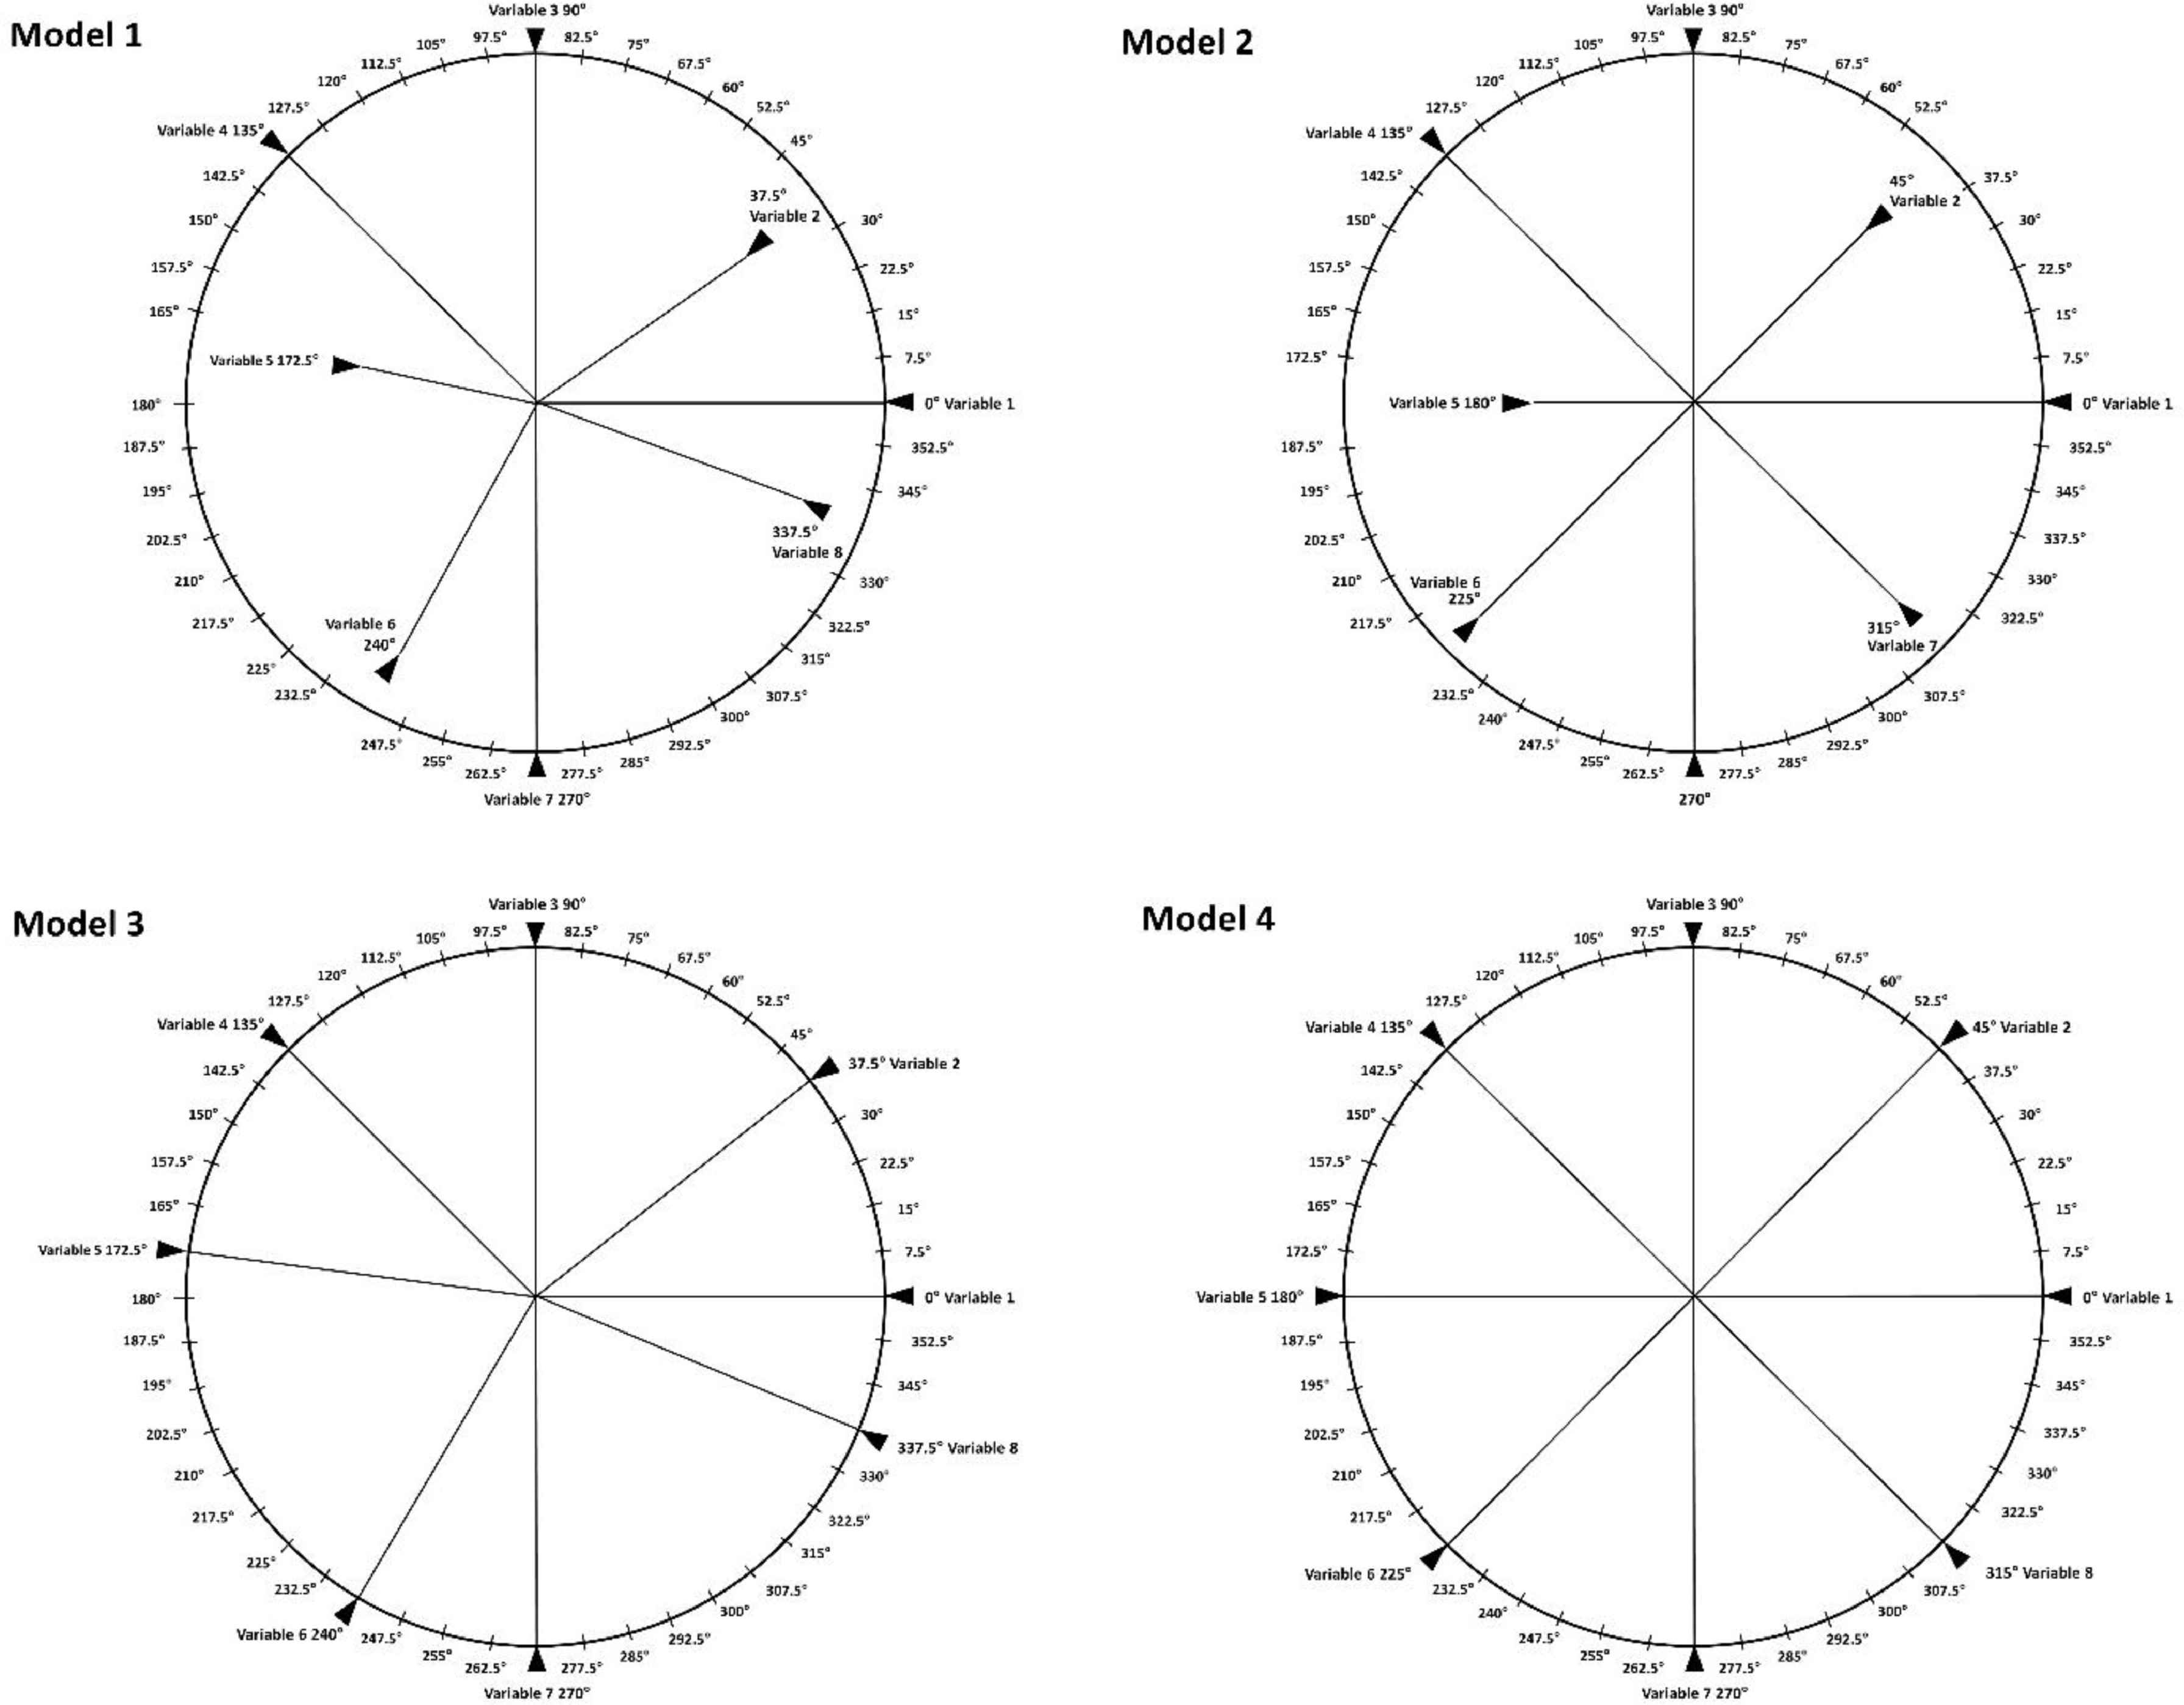
\includegraphics[width=1\linewidth,height=\textheight,keepaspectratio]{figures/Rogoza2021three-fig1.jpg}

}

\caption[\label{fig-rogoza}Graphical representation of four variations
of circumplex model structure. Model 1 is a circular model, Model 2 is a
quasi-circumplex model with equal spacing, Model 3 is a quasi-circumplex
model with equal communality, and Model 4 is a circumplex model with
equal spacing and equal communality.]{\label{fig-rogoza}Graphical representation of four variations
of circumplex model structure. Model 1 is a circular model, Model 2 is a
quasi-circumplex model with equal spacing, Model 3 is a quasi-circumplex
model with equal communality, and Model 4 is a circumplex model with
equal spacing and equal communality.\footnotemark{}}

\end{figure}%
\footnotetext{Reproduced from (Rogoza,
  Cieciuch, and Strus 2021) with permission by the publisher.}

\subsection{Translating circumplex
instruments}\label{translating-circumplex-instruments}

Typically, circumplex scales are measured via a series of questions in a
survey instrument. These instruments are initially developed in one
language and the validity and structure of the instrument is tested in
that language. Often these instruments are directly translated into
other languages to enable their use in other countries. However, the
validity of the instrument in the new language is not guaranteed.
Changes in the correlation structure can be caused by errors in the
translation process, by semantic and linguistic differences between the
translated scales even given a valid translation, and by a lack of
generalisability of the circumplex instrument.

It is easy to see how errors in the translation process can lead to
changes in the correlation structure. For example, if a question is
mistranslated, then the responses to that question will not be
correlated with the responses to the other questions in the instrument.
Semantic and linguistic differences between the translated scales can
also lead to changes in the correlation structure. For example, if a
question is translated into a language where the concept does not exist
or cannot be easily expressed, then the responses to that question will
not be correlated with the responses to the other questions in the
instrument. Finally, it may be that even if the original instrument is
valid for e.g.~the English-speaking population, it may not be valid for
other populations due to cultural differences.

\subsubsection{Goals of translating a circumplex
instrument}\label{goals-of-translating-a-circumplex-instrument}

Two approaches could be taken when attempting to translate a survey
instrument. The first approach would attempt to achieve direct
concurrence with the original instrument, where each scale is directly
correlated with the corresponding scale from the original instrument. If
the circumplex structure is identical between the two languages, then
this approach would allow for the most direct comparison between the two
languages. However, if the circumplex structure is not identical between
the two languages, then this approach would lead to a loss of
information. The second approach would attempt to achieve the same
circumplex structure in the new language as in the original language.
This approach would allow for the most direct comparison between the two
languages.

In this second approach, identifying the differences in structure
between translations enable the process of locating an external variable
to be corrected for the differences in structure. Given that at minimum
a quasi-circumplex structure can be confirmed, then the deviations in
either the angles or communalities from the ideal circumplex structure
can be measured and accounted for. When this is done separately for the
origianl and translated instruments, then an external variable which has
the same theoretical location in both instruments should be located in
the same location in both corrected instruments.

This has an important impact on comparing results under the two
translations. If an external variable is theoretically located in a
single, fixed position in the circumplex space, locating it without
accounting for the differences in structure between the two translations
will lead to different locations in the two translations. The
interpretation of this result would then be that the external variable
is located in different positions in the two languages. However, if the
differences in structure are accounted for, then the external variable
should be located in the same position in both translations. By applying
the correction we can attempt to discover differences in the effect of
external variables, independent of the differences in structure between
the two translations.

\section{A four step procedure for the analysis of circumplex
models}\label{a-four-step-procedure-for-the-analysis-of-circumplex-models}

This section of the Supplementary Material is intended as an extended
companion to Section 3. Data Analysis of the main manuscript. Some text
is repeated here, but additional rationales and details are included
which were ommitted from the manuscript for conciseness.

In Rogoza, Cieciuch, and Strus (2021), the authors propose a three-step
procedure for assessing circumplex models. The steps in this procedure
are: 1) ``verify whether the analzed model is circumplex or not'' using
Structural Equation Modelling based on Browne (1992)'s model; 2) ``test
the possibility to locate an external variable within empirical
circumplex'' using the Structural Summary Method (Gurtman 1994); and 3)
``assess the extent of which empirical locations are in congruence to
the theoretical predictions within the circumplex structure'' (Rogoza,
Cieciuch, and Strus 2021).

We expand upon the three-step procedure proposed by Rogoza, Cieciuch,
and Strus (2021) and adapt it to the specific case of testing multiple
variations (i.e.~translations) of the same circumplex instrument. The
goals of this procedure are, for each translation, to verify the
quasi-circumplex structure of the instrument, to derive angle
corrections, and to test the congruence between the corrected circumplex
and the theoretical circumplex structure. We do this by first adding an
initial step to incorporate Rounds et al. (2000)'s test of the circular
ordering of the scales to confirm that the order of the scales is
maintained across translations. We then follow the same three steps as
Rogoza, Cieciuch, and Strus (2021), but we adapt the third step to test
the congruence between the circumplex structure of the original
instrument and the circumplex structure of the translated instruments
and to allow for adjustments to be made by extracting adjusted angles
from the SEM step.

\subsection{Step 1: Confirm the circular ordering of the circumplex
scales}\label{step-1-confirm-the-circular-ordering-of-the-circumplex-scales}

In line with the procedure taken in Gurtman and Pincus (2000) and
previously employed for the SCM by Lam et al. (2022), we begin by
confirming the circular ordering of the circumplex scales. This test,
developed by Rounds et al. (2000), the test of the circular order model
involves comparing the obtained order relations for a set of scales
against their hypothesized order given a certain circular model. This
test is applied in order to ensure that the process of translation has
not altered the order of the scales and so the test is applied against
the order of the scales in the original instrument. The test is applied
to each translation separately, and the results are compiled into a
single table.

The index used for this test is Hubert and Arabie (1987)'s
correspondence index (CI). This offers a descriptive measure reflecting
the degree to which the model's ordered predictions align with a
specific sample matrix. The metric is calculated as the proportion of
predictions met minus the proportion violated, yielding a range from 1.0
(indicating complete prediction fulfillment) to -1.0 (indicating all
predictions contradicted). In alignment with the methodology outlined by
Tracey (1997), we applied a randomization test to the hypothesized order
relations (Hubert and Arabie 1987), producing an exact probability,
determining the likelihood of achieving the observed model fit in
relation to all potential permutations of the matrix. The index
thresholds for this test are: a p-value \textless{} 0.05 and a CI
\textgreater{} 0.70.

\subsection{Step 2: Confirm the quasi-circumplex structure of the
circumplex
scales}\label{step-2-confirm-the-quasi-circumplex-structure-of-the-circumplex-scales}

We confirm the structure of the circumplex instrument by applying Browne
(1992)'s circular stochastic process model with a Fourier series
correlation function. This model represents a non-standard Structural
Equation Model (SEM) specifically tailored to testing circumplex
structures which allows a researcher to examine the extent to which the
underlying structure of a sample correlation matrix conforms to a
circumplex pattern. The four model variations (unconstrained circular,
equal spacing quasi-circumplex, equal-communality quasi-circumplex, and
strict circumplex with equal spacing and communality) can each be
investigated using this model. For the unconstrained and
quasi-circumplex models, Browne's model allows for the estimation of the
angles and communalities of the circumplex scales. From these results
for the quasi-circumplex models, we can derive the corrected angles for
each translation, which can be used in the next step of the analysis.

This model is implemented in the CircE package (Grassi, Luccio, and Blas
2010) for R (R Core Team 2018)\footnote{The version of CircE originally
  developed by Grassi is no longer maintained and fails on installation
  in R. As such, the specific version of CircE with bug fixes
  implemented by the authors used for this analysis is hosted separately
  on Github at: \url{https://github.com/MitchellAcoustics/CircE-R}}. The
model is applied to each translation separately, testing each of the
four model variations, and the results are compiled into a single table.
CircE provides a suite suite of SEM fit indices, which are statistical
measures used to evaluate the goodness of fit of the models. For this
study, we use the following fit indices: Comparative Fit Index (CFI),
Goodness of Fit Index (GFI), and Standardized Root Mean Square Residual
(SRMR), summarised with their respective thresholds in
Table~\ref{tbl-indices}.

Readers might note that these indices differ slightly from those used by
Rogoza, Cieciuch, and Strus (2021), most notably the exclusion of the
Root Mean Square Error of Approximation (RMSEA), a commonly used metric.
RMSEA was excluded from the analysis on the basis of both Rogoza's own
critiques\footnote{``it is worth noting that the RMSEA may not be best
  suited to evaluate circumplex models. It becomes biased in the case of
  high correlations between proximal variables, as found in circumplex
  models, and should be interpreted with caution.'' (Rogoza, Cieciuch,
  and Strus 2021)} and recent warnings from West et al. (2023).

\begin{longtable}[]{@{}
  >{\raggedright\arraybackslash}p{(\linewidth - 4\tabcolsep) * \real{0.5106}}
  >{\centering\arraybackslash}p{(\linewidth - 4\tabcolsep) * \real{0.1809}}
  >{\centering\arraybackslash}p{(\linewidth - 4\tabcolsep) * \real{0.2979}}@{}}
\caption{Fit indices and thresholds, including the reference from which
the threshold is derived.}\label{tbl-indices}\tabularnewline
\toprule\noalign{}
\begin{minipage}[b]{\linewidth}\raggedright
\textbf{Fit Index}
\end{minipage} & \begin{minipage}[b]{\linewidth}\centering
\textbf{Threshold}
\end{minipage} & \begin{minipage}[b]{\linewidth}\centering
\textbf{Reference}
\end{minipage} \\
\midrule\noalign{}
\endfirsthead
\toprule\noalign{}
\begin{minipage}[b]{\linewidth}\raggedright
\textbf{Fit Index}
\end{minipage} & \begin{minipage}[b]{\linewidth}\centering
\textbf{Threshold}
\end{minipage} & \begin{minipage}[b]{\linewidth}\centering
\textbf{Reference}
\end{minipage} \\
\midrule\noalign{}
\endhead
\bottomrule\noalign{}
\endlastfoot
Correspondence Index (CI) & p \textless{} 0.05,

CI \textgreater{} 0.70 & Gurtman and Pincus (2000) \\
Comparative Fit Index (CFI) & \emph{0.92} & Moshona, Lepa, and Fiebig
(2023) \\
Goodness of Fit Index (GFI) & \emph{0.90} & Rogoza, Cieciuch, and Strus
(2021) \\
Standardized Root Mean Square Residual (SRMR) & \emph{0.08} & Hu and
Bentler (1999)

Moshona, Lepa, and Fiebig (2023)

Tarlao, Steffens, and Guastavino (2020) \\
\end{longtable}

Once each of the model variations are assessed against the above fit
indices, we can determine whether that model variation is a good fit for
the data. If the strict circumplex model meets the fit thresholds across
the translations tested, then the procedure can be continued and no
adjustment will be needed. If, however, the structure of some or all of
the translations are found to have a quasi-circumplex structure, then
adjustments will need to be derived and applied to ensure
cross-comparability between the translated instruments. If the model
variation for the equal-communality model (where the angles are allowed
to vary) is a good fit for the data, then we can use the derived angles
from CircE as adjustments to the circumplex structure.

Importantly, this table also reports the derived angles for each scale
for the unconstrained and Equal comm. models. These angles will be
carried over and used in the next stage of the analysis, where we will
validate the survey instrument by correlating the survey responses with
the acoustic indices using the Structural Summary Method (SSM).

\subsection{Step 3: Locate the full dataset circumplex scales within
each language's circumplex
space}\label{step-3-locate-the-full-dataset-circumplex-scales-within-each-languages-circumplex-space}

Once the general circumplex structure is tested, it is possible to
investigate the likelihood to locate an external variable (this could be
an objective feature such as sound level dB or it could be another
perceptual or psychometric variable such as tranquility) within the
empirical circumplex. The circumplex model provides a precise framework
for predicting the relationships between an external variable and all
circumplex variables. The Structural Summary Method (SSM) is a technique
used to summarize correlation patterns among measurement scores that are
hypothesized to conform to a circumplex structure (Rogoza, Cieciuch, and
Strus 2021). SSM aims to fit a sinusoidal curve to data points (\(q_i\))
based on their nominal angular positions (\(\theta_i\)). This is
achieved by optimizing the parameters for elevation (\(e\)), amplitude
(\(i\)), and displacement (\(d\)). Mathematically, these parameters are
used to model the correlational information (\(q_i\)) in
Equation~\ref{eq-ssm}:

\begin{equation}\phantomsection\label{eq-ssm}{
q_i = e + \alpha cos(\theta_i - d)
}\end{equation}

SSM analysis yields several key estimations, including:

\begin{itemize}
\tightlist
\item
  Model fit (R2), which assesses how well the observed sinusoidal curve
  aligns with the cosine function, indicating the goodness of fit.
\item
  Elevation, representing the average correlation between an external
  variable and all circumplex variables.
\item
  Amplitude (vector length), measuring the distance from the mean of the
  external variable's correlation to its peak correlation with
  circumplex variables. This value signifies the uniqueness of the
  profile, indicating whether it is prominently associated with a
  specific circumplex variable or equally related to all.
\item
  Angular displacement, denoting the angle at which the profile reaches
  its maximum point, indicating the empirical location of the variable
  within the circumplex as observed in the data.
\end{itemize}

\begin{quote}
It is essential to evaluate how well the sinusoidal curve aligns with
the cosine function by examining its goodness of fit, as indicated by
the \(R^2\) value. If \(R^2\) values fall below 0.70, it is advisable
not to interpret the remaining coefficients and to discontinue the
process of locating external variables. Conversely, \(R^2\) values
exceeding 0.80 indicate a strong fit. Additionally, it's worth
mentioning that amplitude estimates, reflecting the distinctiveness of
the profile, and elevation estimates, indicating the presence of a
general factor, are considered notable when they surpass 0.15.
\end{quote}

As described in Rogoza, Cieciuch, and Strus (2021), Step Two involves
testing whether external variables can be located within the circumplex.
Because we have derived new angles in the SEM step, we use these
`adjusted' angles for calculating the SSM parameters. In order to
determine whether the language circumplexes can adequately allow an
external variable to be located, we use the following criteria:

\begin{itemize}
\tightlist
\item
  \(R^2\) \textgreater{} 0.8
\item
  amplitude \textgreater{} .15
\end{itemize}

These indices are based on the criteria used by Rogoza, Cieciuch, and
Strus (2021), however we use an increased criterion of \(R^2 > 0.9\)
since we have a prior expectation that the circumplex variables should
fit very well within each translation's circumplex.

The structure of the circumplex is key to determining where external
variables are located. Given differing angles and communalities, the
external variable can occupy different locations within the circumplex.
Revealing and validating the true structure of a particular circumplex
model is therefore key to reliably identifying correct location of
external variables within the circumplex space.

\subsection{Step 4: Accurately locating circumplex items within each
language}\label{step-4-accurately-locating-circumplex-items-within-each-language}

The final step of Rogoza, Cieciuch, and Strus (2021)'s three step
procedure is to test the congruence between the empirical locations and
theoretical expectations within the circumplex structure. In the case of
the soundscape circumplex and our SATP data, we don't have an external
variable with a defined theoretical location within the circumplex - for
instance loudness does not have a defined location within the circumplex
where it is expected to be located.

Taking inspiration from Yik and Russell (2004), we propose to use the
circumplex structure of the soundscape survey itself as the theoretical
expectation. Yik and Russell (2004) proposes that one circumplex can be
located within another by calculating the SSM correlation between each
of the scales of the reference circumplex and the test circumplex. In
this way, each scale of the reference circumplex can be located within
the test circumplex, and we can test whether these empirical locations
meet our expectations.

The process to do this is as follows:

\begin{enumerate}
\def\labelenumi{\arabic{enumi}.}
\tightlist
\item
  For both the reference and test circumplex, calculate the mean value
  of each scale for each recording.
\item
  Calculate the SSM correlation between each scale of the reference
  circumplex and the test circumplex, in our case using the corrected
  angles.
\item
  Test the congruence betwen the empirical locations and theoretical
  expectations using the Procrustes congruence test (Rogoza, Cieciuch,
  and Strus 2021).
\end{enumerate}

We will be using the full dataset as the reference set and the data from
each translation as the test set. This effectively means that we are
testing whether each translation is able to locate the circumplex
structure of the soundscape survey, consistently across all languages.

This aligns with the overall goal of our process of allowing data
(i.e.~the circumplex coordinate) from different languages to be directly
compared, by correcting for the differences in the circumplex structure
between languages.

\subsubsection{Congruence}\label{congruence}

What Rogoza, Cieciuch, and Strus (2021) (and Orthosim) refer to as
Tucker's Congruence Coefficient is also commonly referred to as the
cosine similarity (see the
\href{https://tensorly.org/stable/modules/generated/tensorly.metrics.factors.congruence_coefficient.html}{Tensorly
documentation}). We therefore use the sklearn implementation of cosine
similarity to calculate the congruence between the empirical locations
and theoretical expectations. This produces a matrix of cosine
similarity values, which we then use to calculate the mean congruence,
to match the model congruence from Rogoza, Cieciuch, and Strus (2021).

\subsubsection{Procrustes}\label{procrustes}

However, it appears that, despite Rogoza, Cieciuch, and Strus (2021) 's
description, this method is not actually based on a Procrustes analysis.
The equivalent distance metric from a Procrustes method would be the
rotational-based Procrustes distance, i.e.~the squared Froebenius norm
of the difference between the two orthogonal matrices. See Andreella et
al. (2023):

\begin{quote}
Instead, the second distance exploits the orthogonal matrix parameters
solution of the Procrustes problem. The rotational-based distance
computes the squared Frobenius distance between these estimated
orthogonal matrices. As we will see, this metric measures the level of
dissimilarity/similarity in orientation between matrices/subjects before
functional alignment.
\end{quote}

Based on the proof given in Bakhtiar and Siswadi (2015), given that the
input matrices are scaled (i.e.~\texttt{rotational(scale=True)}), then
the Procrustes distance is a true distance measure which obeys
\(0 < p(X, Y) < 1\) (Bakhtiar and Siswadi 2015) (p.~322). Therefore we
can convert the Procrustes distance to a similarity measure by
subtracting it from 1.

\phantomsection\label{refs}
\begin{CSLReferences}{1}{0}
\bibitem[\citeproctext]{ref-Andreella2023Procrustes}
Andreella, Angela, Riccardo De Santis, Anna Vesely, and Livio Finos.
2023. {``Procrustes-Based Distances for Exploring Between-Matrices
Similarity.''} \emph{Statistical Methods and Applications} 32 (3):
867--82. \url{https://doi.org/10.1007/s10260-023-00689-y}.

\bibitem[\citeproctext]{ref-Bakhtiar2015symmetrical}
Bakhtiar, T., and Siswadi Siswadi. 2015. {``On the Symmetrical Property
of Procrustes Measure of Distance.''} \emph{International Journal of
Pure and Apllied Mathematics} 99 (3).
\url{https://doi.org/10.12732/ijpam.v99i3.7}.

\bibitem[\citeproctext]{ref-Browne1992Circumplex}
Browne, Michael W. 1992. {``Circumplex Models for Correlation
Matrices.''} \emph{Psychometrika} 57 (4): 469--97.
\url{https://doi.org/10.1007/bf02294416}.

\bibitem[\citeproctext]{ref-Grassi2010CircE}
Grassi, Michele, Riccardo Luccio, and Lisa Di Blas. 2010. {``{CircE}: An
r Implementation of Browne's Circular Stochastic Process Model.''}
\emph{Behavior Research Methods} 42 (1): 55--73.
\url{https://doi.org/10.3758/brm.42.1.55}.

\bibitem[\citeproctext]{ref-Gurtman1994differentiating}
Gurtman, Michael B. 1994. {``Differentiating Normal and Abnormal
Personality.''} In, edited by S. Strack and M. Lorr, 243--63. New York,
NY, US: Springer Publishing Company.

\bibitem[\citeproctext]{ref-Gurtman2000Interpersonal}
Gurtman, Michael B., and Aaron L. Pincus. 2000. {``Interpersonal
Adjective Scales: Confirmation of Circumplex Structure from Multiple
Perspectives.''} \emph{Personality and Social Psychology Bulletin} 26
(3): 374--84. \url{https://doi.org/10.1177/0146167200265009}.

\bibitem[\citeproctext]{ref-Guttman1954new}
Guttman, Louis. 1954. {``A New Approach to Factor Analysis: The
Radex.''} In \emph{Mathematical Thinking in the Social Sciences.},
258--348. New York, NY, US: Free Press.

\bibitem[\citeproctext]{ref-Hu1999Cutoff}
Hu, Li‐tze, and Peter M. Bentler. 1999. {``Cutoff Criteria for Fit
Indexes in Covariance Structure Analysis: Conventional Criteria Versus
New Alternatives.''} \emph{Structural Equation Modeling: A
Multidisciplinary Journal} 6 (1): 1--55.
\url{https://doi.org/10.1080/10705519909540118}.

\bibitem[\citeproctext]{ref-Hubert1987Evaluating}
Hubert, Lawrence, and Phipps Arabie. 1987. {``Evaluating Order
Hypothesis Within Proximity Matrices.''} \emph{Psychological Bulletin}
102 (1): 172--78.
\url{https://oce.ovid.com/article/00006823-198707000-00013/HTML}.

\bibitem[\citeproctext]{ref-Lam2022Assessing}
Lam, Bhan, Esther Monica Peijin Fan, Kenneth Ooi, Zhen-Ting Ong, Joo
Young Hong, Woon-Seng Gan, and Shin Yuh Ang. 2022. {``Assessing the
Perceived Indoor Acoustic Environment Quality Across Building Occupants
in a Tertiary-Care Public Hospital in Singapore.''} \emph{Building and
Environment} 222 (August): 109403.
\url{https://doi.org/10.1016/j.buildenv.2022.109403}.

\bibitem[\citeproctext]{ref-Moshona2023Optimization}
Moshona, Cleopatra Christina, Steffen Lepa, and André Fiebig. 2023.
{``Optimization Strategies for the German Version of the Soundscape
Affective Quality Instrument.''} \emph{Applied Acoustics} 207 (May):
109338. \url{https://doi.org/10.1016/j.apacoust.2023.109338}.

\bibitem[\citeproctext]{ref-RCT2018R}
R Core Team. 2018. \emph{{R}: {A} {L}anguage and {E}nvironment for
{S}tatistical {C}omputing}. Vienna, Austria: R Foundation for
Statistical Computing. \url{https://www.R-project.org/}.

\bibitem[\citeproctext]{ref-Rogoza2021three}
Rogoza, Radosław, Jan Cieciuch, and Włodzimierz Strus. 2021. {``A
Three-Step Procedure for Analysis of Circumplex Models: An Example of
Narcissism Located Within the Circumplex of Personality Metatraits.''}
\emph{Personality and Individual Differences} 169 (February): 109775.
\url{https://doi.org/10.1016/j.paid.2019.109775}.

\bibitem[\citeproctext]{ref-Rounds2000Tinsley}
Rounds, James, Molly C. McKenna, Lawrence Hubert, and Susan X Day. 2000.
{``Tinsley on Holland: A Misshapen Argument.''} \emph{Journal of
Vocational Behavior} 56 (2): 205--15.
\url{https://doi.org/10.1006/jvbe.1999.1738}.

\bibitem[\citeproctext]{ref-Tarlao2020Investigating}
Tarlao, Cynthia, Jochen Steffens, and Catherine Guastavino. 2020.
{``Investigating Contextual Influences on Urban Soundscape Evaluations
with Structural Equation Modeling.''} \emph{Building and Environment}
188 (November). \url{https://doi.org/10.1016/j.buildenv.2020.107490}.

\bibitem[\citeproctext]{ref-Tracey1997RANDALL}
Tracey, Terence J. G. 1997. {``RANDALL: A Microsoft FORTRAN Program for
a Randomization Test of Hypothesized Order Relations.''}
\emph{Educational and Psychological Measurement} 57 (1): 164--68.
\url{https://doi.org/10.1177/0013164497057001012}.

\bibitem[\citeproctext]{ref-West2022Handbook}
West, Stephen G., Wei Wu, Daniel McNeish, and Andrea Savord. 2023.
{``Handbook of {S}tructural {E}quation {M}odeling.''} In, edited by Rick
H. Hoyle, Second, 184--205. New York, NY: Guilford Publications.

\bibitem[\citeproctext]{ref-Yik2004Relationship}
Yik, Michelle S. M., and James A. Russell. 2004. {``On the Relationship
Between Circumplexes: Affect and Wiggins' IAS.''} \emph{Multivariate
Behavioral Research} 39 (2): 203--30.
\url{https://doi.org/10.1207/s15327906mbr3902_4}.

\end{CSLReferences}




\end{document}
